%%%%%%%%%%%%%%%%%%%%%%%%%%%%%%%%%%%%%%%%%%%%%%%%%%%%%%%%%%%%%%%%%%%%%%%%%%%%%%%%
%% Title (en): Multiagent Systems and Organizations                           %%
%% Title (cs): Multiagentní systémy a organizace                              %%
%%                                                                            %%
%% Author: Bc. Lukáš Kúdela                                                   %%
%% Supervisor: Prof. RNDr. Petr Štěpánek, DrSc.                               %%
%%                                                                            %%
%% Academic year: 2011/2012                                                   %%
%%%%%%%%%%%%%%%%%%%%%%%%%%%%%%%%%%%%%%%%%%%%%%%%%%%%%%%%%%%%%%%%%%%%%%%%%%%%%%%%

\chapter{Modelling Organizations -- Platform-Independent Metamodel -- Thespian}

In this chapter we will describe Thespian - our attempt at a platform independent metamodel (PIMM) for organization-centric multiagent systems (OCMASs).

% Platform-idenpendent model
In software engineering, \textit{platform-independent model} (PIM) is a model of a software system, that is independent of the specific technological platform used to implement it.
%\cite{Wikipedia-PlatformIndependentModel}
The main motivation to use a PIM is to build the model once and then automatically transform it to any number of platform-specific models (PSMs) for different (ALT: various) deployment platforms.

% Thespian name inspiration - Thespis of Icaria
Thespian is named after \textit{Thespis of Icaria} (present-day Dionysos, Greece), who lived in the 6th century BC and, according to certain Ancient Greece sources and especially Aristotle, was the first person ever to appear on stage as an actor playing a character in a play (instead of (ALT: as opposed to) speaking as himself) \cite{Wikipedia-Thespis}.

% Thespian inspiration - Aalaadin, O&P, PIM4Agents and powerJade
Thespian is inspired by all four metamodels introduced in the previous chapter: Aalaadin, O\&P, PIM4Agents and powerJade.
Similarly to Aalaadin, it contains both dynamic and static concepts (called \textit{core} and \textit{methodological} concepts in Aalaadin). Instances of dynamic/static concepts will end up as run-time/design-time entities in the platform-specific model.
Like O\&P, it can be used to model holonic MASes.
Similarly to PIM4Agents, it enables explicit modelling of protocol and messages exchanged in these protocols (ALT: in them). 
And finally like powerJade, it is able to represent competences (powers) and responsibilities (requirements) of roles.

% Two partitions: {organization, player and protocol}, {desgn-time and run-time}
The Thespian metamodel can be partitioned in two orthogonal ways: in a high-level and low-level way.
Both partitions will be described in the following sections; the integrated metamodel will be presented in the last section.

% High-level partition
The high-level partition divides the concepts according to the area they represent: organization, player or protocol.
This is a more natural partition of the two since fewer dependencies among concepts from different parts exists than in the other partition.
The organization/protocol part of the MAS can be designed (and implemented) independently of the player part; indeed agent developed by one team can become members of organizations and play roles developed by another team. 

% Low-level partition
The low-level partition separates the concepts based on whether they represent design-time or run-time entities.
The design-time entities are created already at design-time and are usually implemented as \textit{agent classes} on the target agent platform (ALT: in the target agent framework); they are analogous to the concept of \textit{Class} in OOP.
The run-time entities are created only at run-time and are usually implemented as \textit{agent instances} on the target agent platform (ALT: in the target agent framework); they are analogous to the concept of \textit{Instance} in OOP.

% Type-token distinction - definition
Before continuing with the presentation of Thespian, it is important to explain the \textit{type-token distinction}.
In disciplines such as philosophy and knowledge representation, the type-token distinction is a distinction that separates a \textit{concept} from objects that are particular \textit{instances} of that concept.
Thespian has been designed to support the type-token distinction and the correct differentiation is a recurring theme in this chapter.

% Type-token distinction - MAS
As an example of the type-token distinction, consider a MAS.
The \textit{specification} of the MAS (its source code) is the \textit{MAS type} and its \textit{manifestation} (a running MAS) is the \textit{MAS token}.
Just like a type can (and usually does) have many tokens, a MAS specification can have multiple manifestations - the same source code can be run many times.

%%%%%%%%%%%%%%%%%%%%%%%%%%%%%%%%%%%%%%%%%%%%%%%%%%%%%%%%%%%%%%%%%%%%%%%%%%%%%%%%
\section{Organization Metamodel}

% Organization metamodel - usage
The Organization metamodel (figure~\ref{figure:thespian-organization-metamodel}) contains concepts whose instances model organizations and roles with their competences and responsibilities.

\subsection*{Organization and Organization Type}

% Type-token distinction - organization
To enable the type-token distinction, Thespian contains concepts for modelling both an \textit{organization type} and an \textit{organization token} - \textit{Organization type} and \textit{Organization} respectively.

% Organization
\textit{Organization} (also called \textit{Organization instance}) is an actual organization in a running MAS; it is a run-time entity.
% Organization - state
It is classified by an \textit{Organization type} which specifies its role structure.
% Organization - note
Note that despite an organization being a run-time entity, it can be declared at design-time, created at MAS start-up and destroyed at MAS shut-down.

% Organization type
\textit{Organization type} (also called \textit{Organization class}) is a class (ALT: family) of organizations sharing the same role structure; it is a design-time entity.
% Organization type - state
It contains a set of \textit{Roles} defining its role structure.
% Organization type - behaviour
It can be instantiated to yield an \textit{Organization}. 

\subsection*{Role and Position}

% Type-token distinction - role
Thespian contains concepts for modelling both an \textit{role type} and \textit{role token} to enable the type-token distinction - \textit{Role} and \textit{Position} respectively.

% Role
\textit{Role} is a role specification within an organization; it is a design-time entity.
% Role - state
It has a set of \textit{Competences} and a set of \textit{Responsibilities} defining its function in its containing \textit{Organization type} and multiplicity differentiating between a \textit{single role}) - one that can not be played by more than one \textit{Player} in an \textit{Organization} - and a \textit{multiple role} - one that can.
Currently, neither Thespian not Thespian4Jade support differentiating between a \textit{mandatory role} - one that has to be played at all times - and an \textit{optional role} - one that does not have to be.

% Position
A \textit{Position} (sometimes called \textit{Role instance}) is a role realization within an actual organization; it is a run-time entity.
% Position - state
It is a realization of \textit{Role} which specifies its competences
It belongs to an \textit{Organization} and is played by a \textit{Player}.
% Position - note
Note that a \textit{Position} it is usually not declared at design-time, it is created when an \textit{Player} starts playing a rule in an \textit{Organization} and destroyed when that \textit{Player} stops doing so (ALT: playing the \textit{Role} in the \textit{Organization}).

\subsection*{Competence and Responsibility}

Let us consider a player playing a role.
As a result of playing the role, the player gains competences a responsibilities associated with that role.

% Competence
\textit{Competence} is an operation a player playing a role \textit{can} can execute as a result of playing that role; it is a design-time entity.
% Competence - state
A \textit{Competence} can require an argument from a player after its invocation (but before its execution), in which case the argument type (a Java type) has to be specified.
Also it can provide a return value to the player after its execution, in which case the return value type (a Java type) has to be specified.

% Figure: Thespian organization metamodel
\begin{figure}[ht]
	\centering
	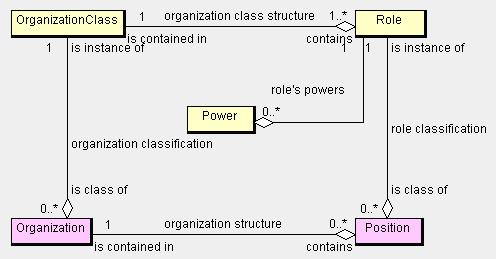
\includegraphics[width=\textwidth]{images/thespian-organization-metamodel.png}
	\caption{The Organization fragment of the Thespian metamodel}
	\label{figure:thespian-organization-metamodel}
\end{figure}

%%%%%%%%%%%%%%%%%%%%%%%%%%%%%%%%%%%%%%%%%%%%%%%%%%%%%%%%%%%%%%%%%%%%%%%%%%%%%%%%
\section{Player Metamodel}

% Player metamodel - usage
The Player metamodel (figure~\ref{figure:thespian-player-metamodel}) contains constructs for modelling players and their responsibilities.

\subsection*{Player and Player Type}

% Type-token distinction - player
To facilitate the type-token distinction, Thespian contains concepts for modelling both a \textit{player type} and a \textit{player token} - \textit{Player type} and \textit{Player} respectively.

% Player
\textit{Player} is an actual player in a running MAS; it is a run-time entity.
% Player - state
It is classified by a player type which specifies its responsibilities.
% Player - note
Note that despite a player being a run-time entity, it has to be declared at design-time, created at MAS start-up and destroyed at MAS shut-down.

% Player type
\textit{Player type} (also called \textit{Player class})is a class (ALT: family) of players sharing the same characteristics, namely responsibilities; it is a design-time entity.
% Player type - state
It has a set of responsibilities defining its capabilities when playing a role.
% Player type - behaviour
It can be instantiated to yield a player. 

\subsection*{Responsibility}

% Responsibility
\textit{Responsibility}is an operation a player playing a role \textit{must} execute as a result of playing that role; it is a design-time entity. 
% Responsibility - state
A \textit{Responsibility} can provide an argument to a player after its invocation (but before its execution), in which case the argument type (a Java type) has to be specified.
Also it can request a return value from the player after its execution, in which case the return value type (a Java type) has to be specified.

% Figure: Thespian player metamodel
\begin{figure}[ht]
	\centering
	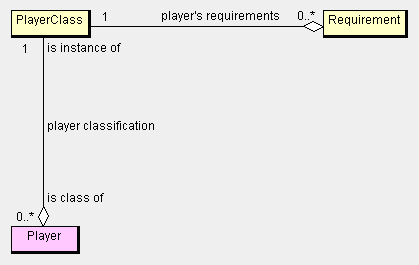
\includegraphics[width=\textwidth]{images/thespian-player-metamodel.png}
	\caption{The Player fragment of the Thespian metamodel}
	\label{figure:thespian-player-metamodel}
\end{figure}

%%%%%%%%%%%%%%%%%%%%%%%%%%%%%%%%%%%%%%%%%%%%%%%%%%%%%%%%%%%%%%%%%%%%%%%%%%%%%%%%
\section{Protocol Metamodel}

% Protocol metamodel - usage
The Protocol metamodel (figure~\ref{figure:thespian-protocol-metamodel}) contains abstractions whose instances represent interaction protocols between a player and an organization or role, and among roles themselves.

\subsection*{Protocol}

% Protocol
An \textit{Interaction protocol} is an institutionalized pattern of interaction (ALT: communication) between two or more roles within an organization; it is a design-time entity modelled by the \textsc{Protocol} class.
It defines parties involved in the interaction and messages exchanged in the communication.

% Scenario
A realization of an interaction (ALT: communication) protocol is an \textit{Interaction scenario} - a sequence of actions performed (ALT: messages exchanged) by two or more roles within an organization; a scenario is a purely run-time entity.
In other words, a protocol is a framework and a scenario (is) one of its possible instantiations.
Since scenarios are usually not (explicitly?) modelled\footnote{Scenarios can be (explicitly?) modelled in snapshots.}, Thespian does not contain the concept of an \textit{Interaction scenario}.

% Type-token distinction - protocol
The theme of type-token distinction is at play here - instances of \textit{Protocol} model \textit{protocol types} and instances of \textit{Scenario} represent \textit{protocol tokens}.

\subsection*{Party}

% Party - definition
A \textit{Party} is a role involved in a protocol; it is a design-time entity modelled by the \textsc{Party} abstract class.
A relationship between roles and protocols is a many-to-many one; a role can participate in multiple protocols and at least two different roles have to take part in a protocol; a party is a reification (embodiment) of this relationship.
% Initiator party & Responder party
A \textit{Party} is either an \textit{Initiator party} - one that initiates the protocol - or a \textit{Responder party} - one that responds to the initiated protocol. These two concepts are modelled by two concrete classes: \textsc{InitiatorParty} and \textsl{ResponderParty} respectively.

\subsection*{Message}

A \textit{Message} is a piece of information exchanged between two parties in a protocol; it is a design-time entity modelled by the \textsc{Message} class.

% Figure: Thespian protocol metamodel
\begin{figure}[ht]
	\centering
	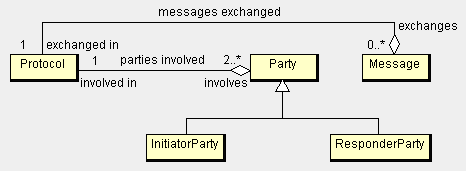
\includegraphics[width=\textwidth]{images/thespian-protocol-metamodel.png}
	\caption{The Protocol fragment of the Thespian metamodel}
	\label{figure:thespian-protocol-metamodel}
\end{figure}

%%%%%%%%%%%%%%%%%%%%%%%%%%%%%%%%%%%%%%%%%%%%%%%%%%%%%%%%%%%%%%%%%%%%%%%%%%%%%%%%
\section{Static (Design-Time) Metamodel}	

% Static metamodel - usage
The Static metamodel contains concepts that represent design-time entities - entities that are created/modified at design-time, i.e. in the MAS source code.

% Figure: Thespian static metamodel
\begin{figure}[ht]
	\centering
	
\includegraphics[width=\textwidth]{images/thespian-static-metamodel.png}
	\caption{The static fragment of the Thespian metamodel}
	\label{figure:thespian-static-metamodel}
\end{figure}

%%%%%%%%%%%%%%%%%%%%%%%%%%%%%%%%%%%%%%%%%%%%%%%%%%%%%%%%%%%%%%%%%%%%%%%%%%%%%%%%
\section{Dynamic (Run-Time) Metamodel}

% Dynamic metamodel - usage
The Dynamic metamodel contains abstractions that abstract dynamic entities - entities that are created/modified at run-rime, i.e. in the actual running MAS.

% Figure: Thespian dynamic metamodel
\begin{figure}[ht]
	\centering
	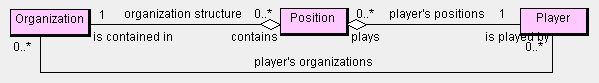
\includegraphics[width=\textwidth]{images/thespian-dynamic-metamodel.png}
	\caption{The dynamic fragment of the Thespian metamodel}
	\label{figure:thespian-dynamic-metamodel}
\end{figure}

%%%%%%%%%%%%%%%%%%%%%%%%%%%%%%%%%%%%%%%%%%%%%%%%%%%%%%%%%%%%%%%%%%%%%%%%%%%%%%%%
\section{Integrated Metamodel}

Figure~\ref{figure:thespian-integrated-metamodel} shows the integrated Thespian metamodel.

% Key property of Thespian - no association between Role and Player type
We would like to emphasize what we perceive as key property of Thespian - there is no association between \textit{Role} and \textit{Player type}, no link between a specific role and a particular player type.
This means that there is no design-time dependency between roles and player types; all connections arise at run-time and happen between positions and players.

% Figure: Thespian integrated metamodel
\begin{figure}[ht]
	\centering
	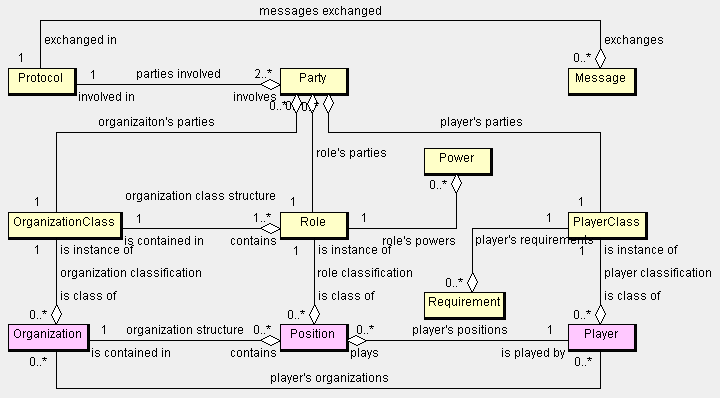
\includegraphics[width=\textwidth]{images/thespian-integrated-metamodel.png}
	\caption{The integrated Thespian metamodel}
	\label{figure:thespian-integrated-metamodel}
\end{figure}